\subsection{Trasduttore di corrente CSLA2CD}

\begin{wrapfigure}[9]{l}{0.4\textwidth}
    \centering
    \includegraphics[scale=0.3]{corrente/csla2cd.png}
\end{wrapfigure}


Il trasduttore di corrente ad effetto Hall \textbf{CSLA2CD} è in grado di misurare la
corrente che lo attraversa senza la necessità di un collegamento fisico con
l'impianto. Il principio di funzionamento si basa sulla misura del campo
magnetico generato dal conduttore (in cui il trasduttore è immerso) piuttosto
che dell'intensità di corrente effettiva. Il passaggio di corrente all'interno
di un conduttore determina infatti la presenza di un campo magnetico avente
linee di campo concentriche e modulo proporzionale all'intensità di corrente.

\vspace{12mm}

Quando alimentato con una tensione di $8V_{DC}$ fornisce un'uscita in tensione sinusoidale con offset del tipo:

\begin{equation}
    V_o = 4 + 0.0327 \cdot I_{picco}
\end{equation}

L'alimentazione a 8V viene realizzata tramite uno stabilizzatore di tensione
LM7808 (come mostrato in figura \ref{fig:8v}) e l'uscita del trasduttore viene disaccoppiata
con un buffer prima di passare al circuito di condizionamento.

\begin{figure}[H]
    \centering
    \begin{subfigure}{0.49\textwidth}
        \centering
        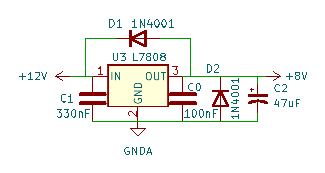
\includegraphics[scale=1.3]{corrente/lm7080.eps}
        \caption{Circuito di alimentazione 8V}
        \label{fig:8v}
    \end{subfigure}
    \begin{subfigure}{0.49\textwidth}
        \centering
        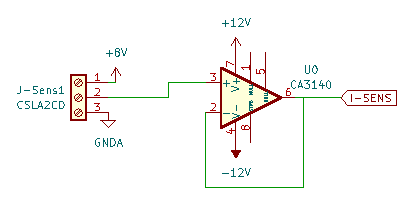
\includegraphics[scale=1.3]{corrente/buffer_csla2cd.eps}
        \caption{Buffer}
    \end{subfigure}
    \caption{Collegamento CSLA2CD}
\end{figure}